%-----------------------------------------------------------------------------
%
%               Template for sigplanconf LaTeX Class
%
% Name:         sigplanconf-template.tex
%
% Purpose:      A template for sigplanconf.cls, which is a LaTeX 2e class
%               file for SIGPLAN conference proceedings.
%
% Guide:        Refer to "Author's Guide to the ACM SIGPLAN Class,"
%               sigplanconf-guide.pdf
%
% Author:       Paul C. Anagnostopoulos
%               Windfall Software
%               978 371-2316
%               paul@windfall.com
%
% Created:      15 February 2005
%
%-----------------------------------------------------------------------------


\documentclass[10pt,nocopyrightspace]{sigplanconf}

% The following \documentclass options may be useful:
%
% 10pt          To set in 10-point type instead of 9-point.
% 11pt          To set in 11-point type instead of 9-point.
% authoryear    To obtain author/year citation style instead of numeric.

\usepackage[normalem]{ulem}
\newcommand{\Comment}[1]{\textcolor{red}{\bf #1}}
%\renewcommand{\iff}{\ensuremath{\mathrm{iff}}}
\usepackage{tabularx}
\usepackage{fancyhdr}
\usepackage{float}
\usepackage{graphicx}
\usepackage{epstopdf}
\usepackage[labelfont=bf]{caption}
\usepackage{subcaption}
\usepackage{natbib}
\usepackage{balance}

\epstopdfsetup{update}

\begin{document}

%\titlebanner{}        % These are ignored unless
\preprintfooter{}   % 'preprint' option specified.

\title{Automatic Pipeline Register Placement Through Delay Backannotation in Chisel}
\subtitle{}

\authorinfo{Wenyu Tang, Donggyu Kim}
           {University of California, Berkeley}
           {\{wenyu, dgkim\}@eecs.berkeley.edu}

\maketitle

\begin{abstract}
We improve the Chisel automatic pipelining tool by automatically optimizing the placement of the pipeline registers. We do this by back annotating Chisel graph nodes with delay data obtained through synthesis and then using this delay information to optimize the placement of the pipeline registers through the use of simulated annealing. 
\end{abstract}

\section{Introduction}
In the existing automatic pipelining tool, the designer can specify the exact placement of the pipeline registers by labeling particular Chisel nodes as pipeline boundary nodes. Alternatively, the designer can label a small subset of the chisel node graph with pipeline stage numbers and have the automatic pipelining tool infer where to place the pipeline registers. In this second method of pipeline specification, the tool will pick some legal pipeline register placement without considering the consequences of the pipeline register placement on critical path delay. A pipeline register placement is legal if every combinational logic node has all of its inputs in the same pipeline stage.

In the second method of specification, we want the automatic pipelining tool to be able to infer not only a legal pipeline register placement, but also a pipeline register placement that optimizes the critical path delay.  This will allow the designer to be able to create a well-balanced pipelined design without repeatedly going through the vlsi design tools to get feedback on critical path length.  Combined with ability of the automatic pipelining tool to automatically generate control logic, the designer will be able to very quickly explore the design space of different pipeline depths and hazard 

\section{Background}
\subsection{Automatic Pipelining}
\label{sec:related-work}
This project is based on the existing automatic pipelining tool built on top of Chisel\cite{Bachrach:2012}. The existing automatic pipelining tool allows the RTL designer to specify a one cycle implementation of a finite state machine along with a set of annotations that specify the pipeline stage number of a subset of Chisel graph nodes in the design. During the Chisel backend elaboration process, the automatic pipelining tool transforms the original one stage implementation of the finite state machine into a pipelined design with the correct hazard resolution logic according to the pipeline stage number annotations. The tool resolves pipeline hazards (which are confined to read-after-write hazards) in one of three ways: interlocking, bypassing, and speculation. The tool resolves pipeline hazards with interlocking by default and the user can select particular state elements to be resolved with bypassing and speculation with additional annotation.

This tool expands upon the work by Nurvitadhi et al~\cite{hoe:syn}, which provided a means to automatically pipeline finite state machines by having the designer label every combinational and sequential node in the design in a hierarchical manner using a specialized specification language. Our automatical pipelining tool does not require the user to annotate every node with a stage number and automatically finds the close-to-optimal pipeline register placements.

\subsection{Chisel Backannotation}

\begin{figure*}
	\centering
    \resizebox{1.5\columnwidth}{!}{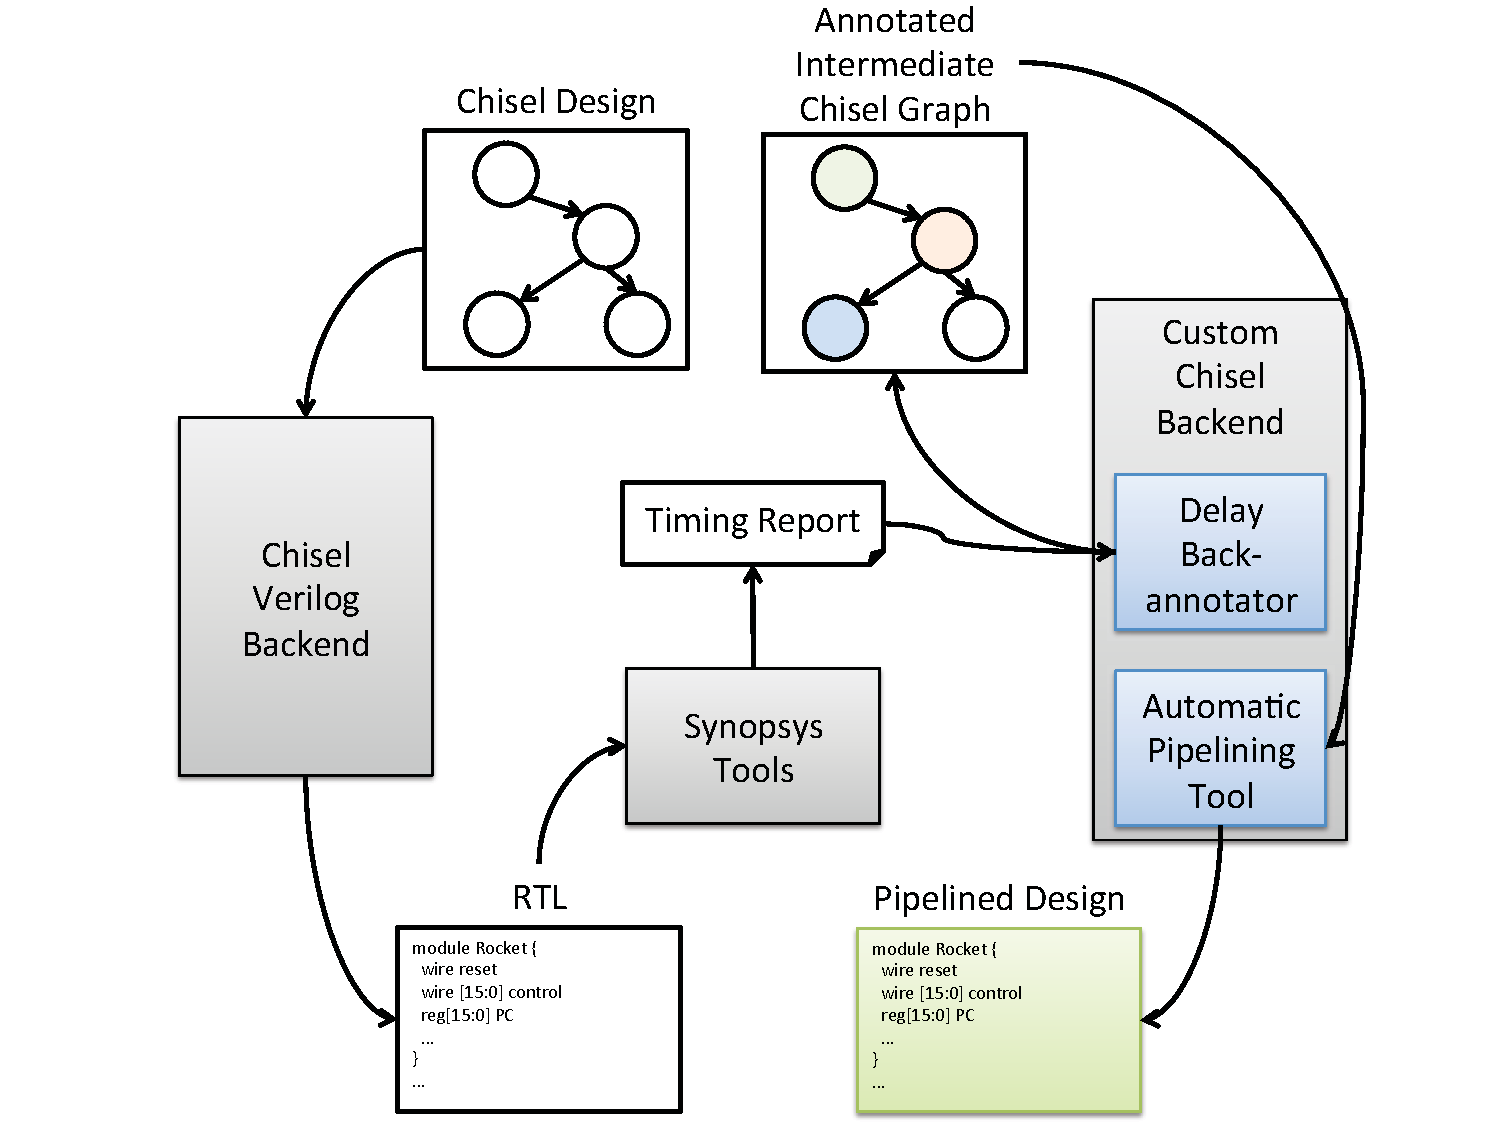
\includegraphics{figures/toolflow}}
    \caption{The overall tool flow}
	\label{fig:toolflow}
\end{figure*}
ßß
\section{Tool Flow}
Figure \ref{fig:toolflow} shows the flow of the entire systems. As the first step, we executes the Chisel Verilog Backend which translates a Chisel design into an RTL. The RTL will be used by Synopsys tools to generate timing reports. This is preparation for the second backend execution.

The second backend execution produces a pipelined design from the original Chisel design. We define a customized Chisel backend to include the delay backannotator and the automatic pipelining tool and then execute it. In the second backend execution, the delay backannotator calls Synopsys tools to produce timing reports. It then annotates the intermediate Chisel graph, which is explained in Section \ref{sec:challenges}, by reading the timing reports. The automatic pipelining tool uses the annotated graph to locate the pipeline registers at the optimal places, producing an automatically pipelined design.
\section{Technical Approach}
% Automatically finding a close-to-optimal placement of the pipeline registers consists of two major processes. First, we backannotate Chisel graph nodes with delay information obtained afelaborationter logic synthesis. Next, we use simulated annealing to place the pipeline registers based on the delay data obtained by the backannotation.

\subsection{Chisel Backannotation}
\begin{table*}
	\centering
	\begin{tabular} 
		{ |c | c| }
		\hline
		\textbf{Origianl backend elaboration flow} & \textbf{Backend elaboration flow for backannotation} \\
		\hline \hline
		\multicolumn{2}{| c |}{{\bf -} Set the top module} \\
		\multicolumn{2}{| c |}{{\bf -} Generate muxes} \\
		\multicolumn{2}{| c |}{{\bf -} Execute pre-elaborate transforms} \\
		\multicolumn{2}{| c |}{{\bf -} Gather and sort child modules} \\
		\multicolumn{2}{| c |}{{\bf -} Assign clocks and resets} \\
		\multicolumn{2}{| c |}{{\bf -} Infer bit-widths} \\
		\hline
		{\bf -} \emph{Remove type nodes} & {\bf -} \emph{Collect nodes into components} \\ 
		\cline{2-2}
		& {\bf Intermediate-level Chisel graph} \\
		& {\bf - } \emph{Name nodes} \\
		& {\bf - } \emph{Assign signal names} \\
		& {\bf - } \emph{Perform backannotation} \\ 
		\cline{2-2}
		{\bf -} \emph{Collect nodes into components} & {\bf -} \emph{Remove type nodes} \\
		\hline
		\multicolumn{2}{| c |}{{\bf -} Execute transforms} \\
		\multicolumn{2}{| c |}{{\bf -} Trace nodes (assign bindings)} \\
		\multicolumn{2}{| c |}{{\bf -} Name nodes} \\
		\multicolumn{2}{| c |}{{\bf -} Execute analyses} \\		
		\multicolumn{2}{| c |}{{\bf -} Find combinational loops } \\
		\hline
		{\bf Verilog translation} & \\
		{\bf -} \emph{Assign signal names} & \\
		\hline
	\end{tabular}
	\caption{Comparison between the original backend elaboration flow and the backend elaboration flow for backannotation. Note that signal names are assigned to intermediate-level Chisel graph nodes while they are given during Verilog translation in the original backend.}
	\label{fig:backend_flow}
\end{table*}

\subsubsection{Challenges and Approaches} 
\label{sec:challenges}
There are several challenges for Chisel backannotation. The first is naming problems, which occurs when the destination nodes have different names. Signal names are given during Verilog translation, a process after the elaboration process and this is highly affected by graph topology. However, other tools like the automatic pipelining tool are expected to manipulate a high-level Chisel graph which goes through only part of the elaboration process, while the Chisel backannotator wants to use a low-level Chisel graph which is elaborated by the backend. The two graphs look different from each other, which makes it difficult to match signal names between them. Thus, we define the intermediate-level Chisel graph so that both the backannotator and the tools are satisfied.

Table \ref{fig:backend_flow} compares the backend elaboration flow for backannotation with the original elaboration flow. \textbf{Remove type nodes} and \textbf{Trace nodes} are processes tools want to avoid because they change the graph topology undesirably. Thus, we apply processes necessary for backannotation to an initial graph prior to \textbf{Remove type nodes} and \textbf{Trace nodes}, and then obtain an intermediate-level Chisel graph. Signal names are assigned to intermediate graph nodes, and backannotation is performed. Tools like the automatic pipelining tool manipulate this backannotated graph.

The second challenge is missing signals during logic synthesis. Missing signals are inevitable although we give signal preserving commands to Synopsys tools. This occurs when Chisel graph nodes are mapped to generic logic blocks by Synopsys tools. These generic logic blocks are replaced by technology-dependent logic cells, and signals of the logics are replaced by arbitrary nets during the compilation of Synopsys tools.

An approach to this problem is calculate the arrival time difference between two non-missing signals in a timing path, and assigning the average value of the difference to missing signals. For example, suppose we have a path from X through T1, T2, and T3 to Y where T1, T2, and T3 are missing signals, and the arrival times of X and Y are 0.1 and 0.5, respectively. The arrival time difference between X and Y is 0.4, and the delays for T1, T2, T3, and Y are estimated as 0.1.

Another challenge is conditional statements like \emph{if} and \emph{switch}. These statements are converted into logic gates during logic synthesis which are not visible in Chisel graphs. Currently, we cannot directly backannotate corresponding nodes in the Chisel graphs with their delays. Instead, there is a separate variable in reset and enable signals of registers. The Chisel backannotator uses this variable to mark the delays of conditional statements.

\subsubsection{Delay Backannotation Flow}
The Chisel backannotator annotates intermediate-level Chisel graph nodes with delay information as follows:

{\bf (1) Finds all possible timing paths}
	
The timing analysis tool finds and analyzes all of the timing paths in the design. The data is launched at the start point of a timing path by a clock edge, propagated through combinational logic in the path, and captured at the endpoint of the path by another clock edge. The startpoint of a path is a clock pin of a sequential element or and an input port of the design. The endpoint is a data input pin of a sequential logic or an output port of the design. 

The Chisel backannotator uses timing path reports to annotate Chisel graphs. It finds all possible timing paths in a Chisel graph to be reported. A timing path is given as a list of Chisel nodes where the start node represents either a register or an input port, the end node represents a register or an output port, and the intermediate nodes represent combinational logics. 

{\bf (2) Generates a tcl script}

A tcl script consists of a set of Synopsys tool commands. For backannotation, it is necessary to generate a customized tcl script to obtain design specific timing path reports. A tcl script generated by the Chisel backannotator contains commands to report timing information of the paths found in Step {\bf (1)}, as well as basic commands to specify libraries, read and compile designs, and write the results. 

{\bf (3) Executes Synopsys tools}

In this step, the Chisel backannotator executes Sysnopsys tools with the tcl script generated by Step {\bf (2)}, which produces timing path reports. Note that the RTL used by Synopsys tools is produced in advance by the first run of the Chisel Verilog backend.

{\bf (4) Reads the timing report and calculates the delays of Chisel nodes}

The timing report produced by Step {\bf (3)} contains 1) the output signals of Chisel nodes (including missing signals) consisting of a timing paths, and 2) the arrival times of nets in the path. The output signal of a Chisel node corresponds to a net in the gate-level netlist, and its arrival time is obtained from the timing report. Thus, the node delay is calculated as the arrival time difference between its output signal and the output signal of its input Chisel graph node.

However, it is impossible to know the arrival times of missing signals because they do not have a corresponding net in the gate netlist. In this step, the chisel backannotator estimates the arrival times of missing signals using the method in Section \ref{sec:challenges}. It also calculates the delays of conditional statements as the arrival time difference between a register and its reset or enable signal.

{\bf (5) Annotates the Chisel graph with the delays}

The Chisel backannotator annotates the intermediate Chisel graph with delays obtained from Step {\bf (4)}.

{\bf (6) Calculates the critical path delay}

In this step, the Chisel backannotator calculates the sum of the Chisel node delays in a timing paths. The critical path is a timing path which has the largest sum. The critical path delay can be used to verify the accuracy of the Chisel backannotator.

\subsection{Automatic Pipeline Register Placement}
The automatic pipelining tool first creates a legal placement of pipeline registers based on the stage numbers of the user annotated nodes and then uses simulated annealing based on the delay data provided by the backannotation to find a close-to-optimal placement of the pipeline registers. 

\subsubsection{Pipeline Legality}
For a pipeline register placement to be legal, it must satisfy the following three conditions:

{\bf (1)} Every combinational logic node has all input signal with the same stage number.  

{\bf (2)} The stage number of every combinational logic node's output signal is equal to the shared stage number of its input signals.

{\bf (3)} There are two ways to determine the stage number of a node. One way is to trace through the node's inputs to a pipeline register and set the stage number of the node equal to the stage number of that pipeline register. Another way is to trace through the node’s consumers to a pipeline register and set the stage number of the node equal to the stage number of that pipeline register {\tt -}  1. For all nodes in the graph, the stage number of the node obtained through both methods must be the same.

\subsubsection{Wire Node Insertion}
\label{wiresection}
Before the automatic pipelining tool infers the initial legal placement of the pipeline registers, it inserts Chisel Bits nodes representing wires between combinational logic nodes in the original design. This ensures that a pipeline boundary never has to fall across a combinational logic node, which would be difficult to reconcile with the notion of Pipeline Legality discussed above.
\subsubsection{Initial Placement}
The automatic pipelining tool breaks cycles in the Chisel graph by splitting architectural registers(registers present in the original one cycle design) into read and write points. The read point consists of the output of the register and the write points consist of the write data and write enables going into the register. Hence, the data sources in the Chisel node graph are read points, input nodes, and constants and the data sinks in the Chisel node are the write points and output node.

Due to reasons that will become apparent from the algorithm discussed below, in general the designer must annotate all of the data sources and data sinks in the Chisel graph in order for the automatic pipelining tool to produce a legal pipeline register placement.

The automatic pipelining tool produces the initial legal pipeline placement by propagating stage numbers out from the user annotated Chisel nodes to their inputs and consumers in a pseudo breadth-first-search (BFS) manner. When two propagation frontiers with different stage numbers meet at the same node, propagation down that path stops and pipeline registers are inserted at that node.

We must maintain the following conditions during the pipeline stage propagation process:

{\bf (1)} Adjust the propagation rates of each propagation frontier so that two different propagation frontiers never meet at a combinational logic node and always meets at a wire node mentioned in \ref{wiresection}, because it does not make sense to split a combinational logic node in half with a pipeline register.

{\bf (2)}  The stage number propagated to a combinational logic node with multiple inputs must be the maximum of the stage numbers of all of its inputs. If this was not maintained, we would have some inputs of the combinational logic node have a greater stage number than the stage number of the output of the combinational node, which violates 2nd condition of Pipeline Legality. This also means that we cannot propagate to a Chisel node with multiple inputs from the input side until all of its inputs have been propagated to.

{\bf (3)} The stage number propagated to a combinational logic node with multiple consumers must be the minimum of the stage numbers of all of its consumers. If this was not maintained, we would have some consumers of the combinational logic node have a smaller stage number than the stage number of the output of the combinational node, which cause that consumer to violate the 3rd condition of Pipeline Legality. This also means that we cannot propagate to a Chisel node with multiple consumers from the consumer side until all of its consumers have been propagated to.

Due to conditions (2) and (3), if not all of the data sources and data sinks are user annotated, the stage propagation process may never complete.
\subsubsection{Optimizing Register Placement}
Once the tool finds an initial legal pipeline register placement, it uses simulated annealing to optimize the placement of the pipeline registers based on the delay data obtained from the Chisel backannotation.

{\bf Simulated Annealing Algorithm}.

We want a fast method of finding a close-to-optimal pipeline register placement without getting stuck at local minimums. Simulated annealing is a gradient decent like algorithm that iteratively improves upon the current solution by randomly generating neighbor solutions from the current solution and then picking the neighboring solution that decreases the cost function the most as the next solution. Unlike gradient decent, simulated annealing occasionally picks neighbor solutions that are worse than the current solution. This allows the algorithm to avoid getting stuck at local minimums. The algorithm uses the following formula to decide if it should choose a neighbor solution as the next solution:
$$
e^{-\Delta cost/T} > R(0,1)
$$

%\begin{figure}[htb]
%\centering
%\resizebox{\columnwidth}{!}{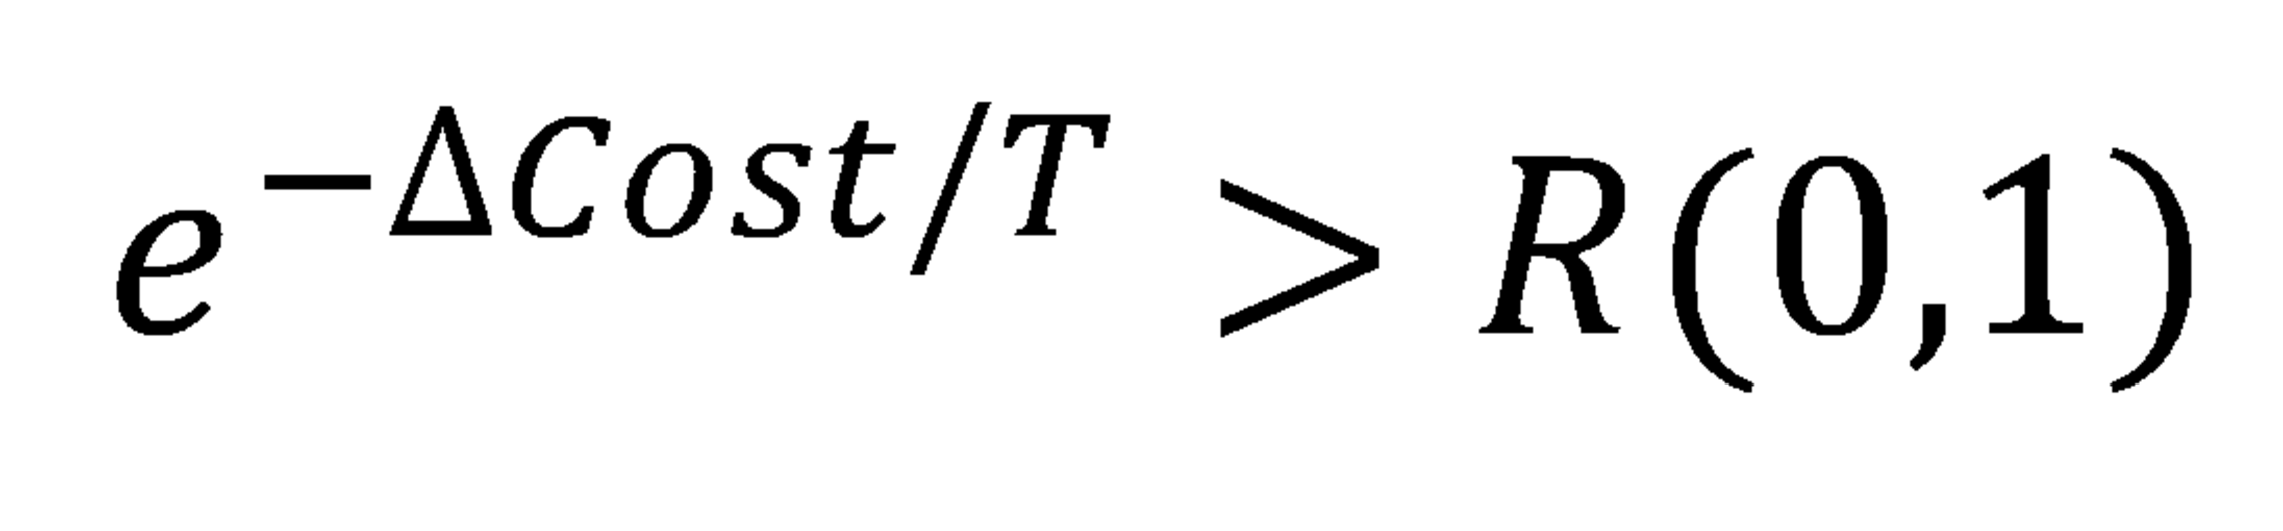
\includegraphics{figures/SimulatedEq.pdf}}
%\end{figure}

$R(0,1)$ is a random number in the interval $[0, 1]$. At higher values of $T$ (temperature), the algorithm is more likely to accept bad solutions. As the algorithm progresses, the value of T is lowered so that the algorithm eventually settles on a close-to-optimal solution. On each iteration, we lower $T$ by $T$ * cooling rate.


This cooling policy forces the algorithm to try many bad solutions in the very early iterations and then focus on trying good solutions for the majority of the remaining iterations. There are many possible cooling schedules, but this one has worked well for us.

We use a starting temperature of 10000 and a cooling rate of 0.002. We terminate the algorithm when the temperature falls below 0.01 or if the iteration count exceeds 3000. We have found the critical path length has generally converged by those two limits in the designs we evaluated.

The cost function used for our problem is the maximum combinational path length in the design and we obtain neighbor solutions from the current solution by moving Chisel nodes across pipeline boundaries in a way that mains a legal pipeline register placement


{\bf Generating Neighbor Solutions}.

We must maintain a legal pipeline register placement as we generate new pipeline register placements from the current pipeline register placement. To accomplish this, we look at the current pipeline register placement and choose eligible combinational logic nodes to move across pipeline stage boundaries. A combinational logic nodes is eligible if it meets the following condition:

{\bf (1)} 
The node is not an architectural register read point, architectural register write point, input node, or output node. We choose to not allow the automatic pipelining tool to move these nodes because doing so could have large unforeseen performance implications. For example, if we are pipelining a RISC processor, moving the write point of the PC register to later stages will cause branches to be resolved later in the pipeline and thus cause a larger branch mispredict penalty.

And one of the following conditions:

{\bf (2)}  
The node outputs directly to a pipeline register. In this case, it is safe to move the node forward across the pipeline boundary by removing the pipeline register from the output of the node and adding pipeline registers to all the inputs of the node and still maintain a legal pipeline register placement. 

{\bf (3)} 
The node has all of its inputs driven directly by a pipeline register. In this case, it is safe to move the node backward across the pipeline boundary by removing the pipeline registers from the inputs of the node and adding a pipeline register to the output of the node and still maintain a legal pipeline register placement.


{\bf Evaluating Cost Function}.

We calculate the longest combinational path in the design by finding the propagation delay to each combinational logic node from an architectural register or pipeline register recursively. The propagation delay to a node is the maximum of (sum of propagation delay to input and delay across input) over all of its inputs. The propagation delay to the output wire of architectural registers and pipeline registers is the clk-to-q delay.  Thus, the longest combinational path is the maximum of the above calculated propagation delay over all nodes in the Chisel graph.

When we generate a new pipeline register placement from the current pipeline register placement, we do not need to recalculate the propagation delay to every node. Instead we store the propagation delays of all the Chisel graph nodes for the current pipeline register placement in a map of Chisel node to propagation delay and incrementally update the map as we modify the pipeline register placement. When we move a combinational logic node forward across a pipeline boundary, we only have to recalculate the propagation delay for the nodes that are newly on the consumer tree of the node that was moved. When we move a combinational logic node backward across a pipeline boundary, we only have to recalculate the propagation delay for the nodes that were previously on the consumer tree of the node that was moved. This allows us to evaluate the cost of new pipeline register placements quickly, even for large designs.



\section{Results}
\begin{figure}
	\centering
    \resizebox{\columnwidth}{!}{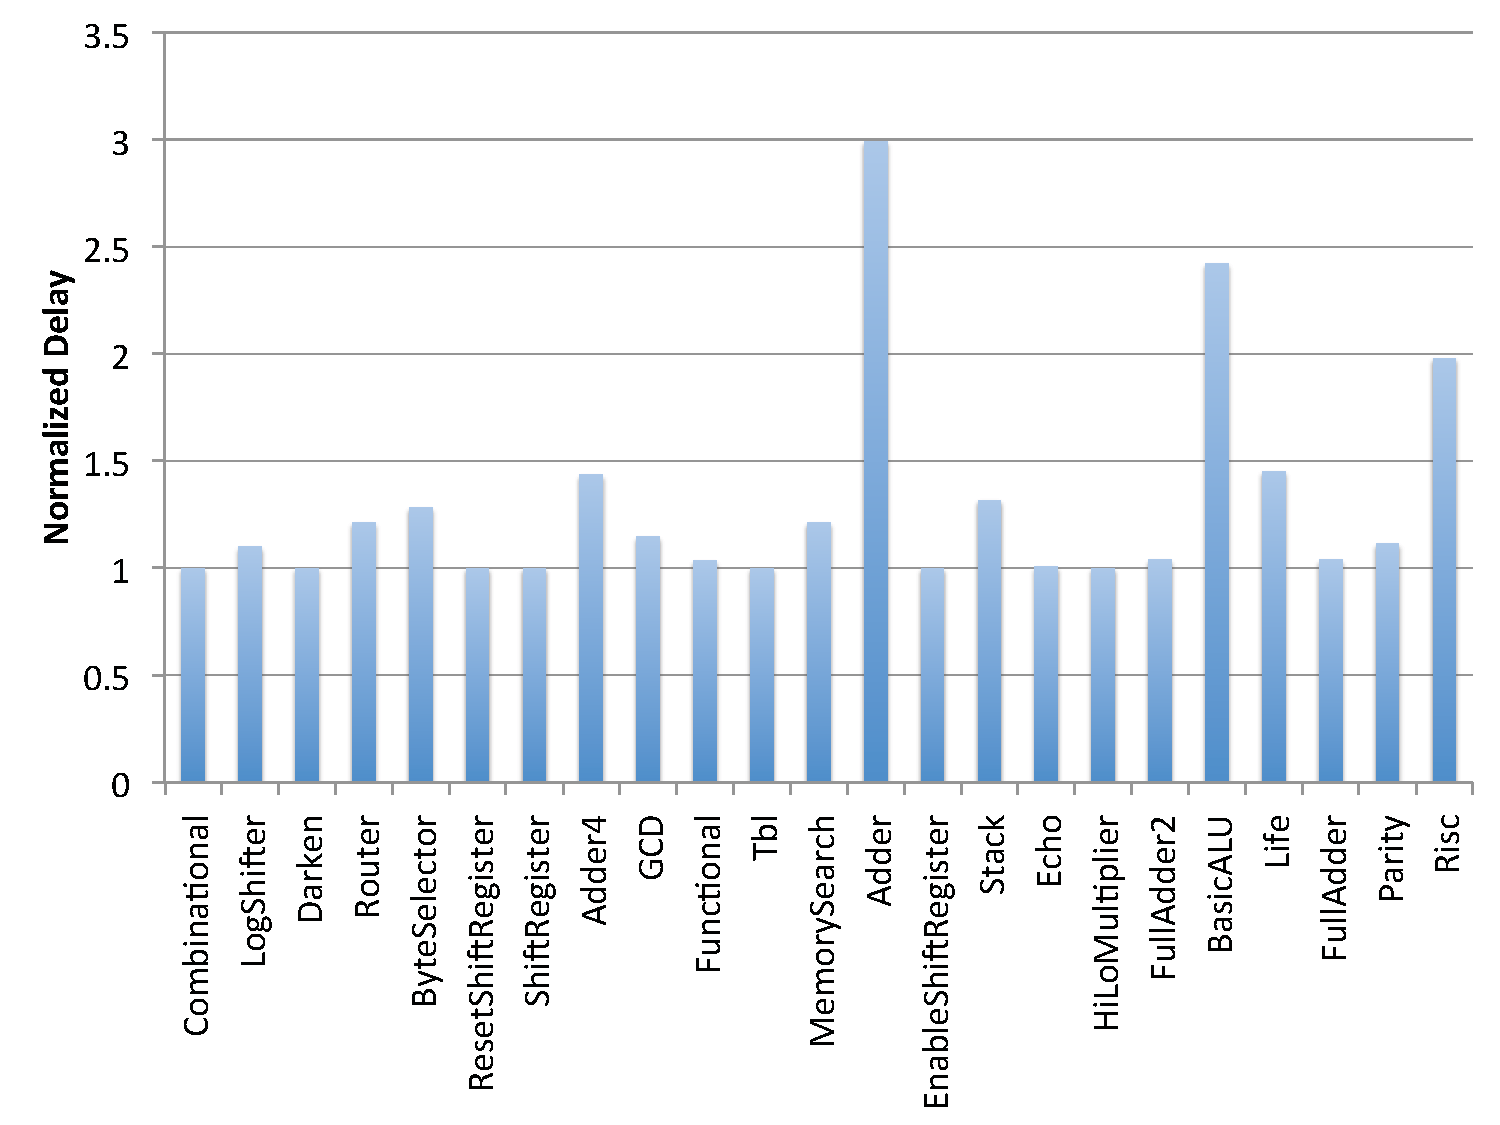
\includegraphics{figures/backannotation_result}}
    \caption{The critical path delays from the Chisel backannotator normalized to those from Design Compiler. We use example Chisel designs in the Chisel tutorial}
	\label{fig:backannotation_result}
\end{figure}
\subsection{Chisel Backannotation}
To verify the Chisel backannotator, we compare the critical path delays from the Chisel backannotator with those from Design Compiler. Figure \ref{fig:backannotation_result} shows the critical path delays calculated by the Chisel backannotator normalized to those calculated by Design Compiler. Design Compiler executes with minimal optimizations, which only checks hold time constraints. With the ideal Chisel backannotator, the normalized critical path delays should be equal to 1. The delays of most designs are very close to 1.

However, those of designs like Adder, BasicALU, and Risc are far away from 1. The inaccuracy of the backannotation mainly comes from the arrival time estimation for missing signals presented in Section \ref{sec:challenges}. It is possible for a Chisel node to have a delay number greater than its actual delay. For example, suppose there are only two timing paths P1 and P2 in the design. P1 is a path from X through T1, T2, and T3 to Y, and P2 is a path from X through T1 and T4 to Y where T1, T2, T3, and T4 are missing signals. We also assume that the delay of P1 is 4 and the delay of P2 is 3.9. In this case, the critical path is P1 whose delay is 4. The Chisel backannotator estimates the arrival times of T1, T2, T3 are 1, 2, 3, respectively, when reading the timing report of P1, while it estimates those of T1, T4 is 1.3, 2,6, respectively, when reading the timing report of P2. The Chisel backannotator concludes the delay of the node whose output signal is T1 or Y is 1.3 and the critical path delay is 4.6. This explains why some designs such as Adder, BasicALU, Risc, and Life have a normalized critical path delay much greater than 1.

To be worse, the fact that a design has a normalized delay equal to 1 does not mean each Chisel node has the exact delay number. This is because the arrival time of missing signals are estimated, which might not affect the critical path delay. For this reason, we need additional accuracy validation for the Chisel backannotator. 

\subsection{Automatic Pipeline Register Placement}
\label{auto_result}

\begin{figure}[htb]
\centering
\resizebox{\columnwidth}{!}{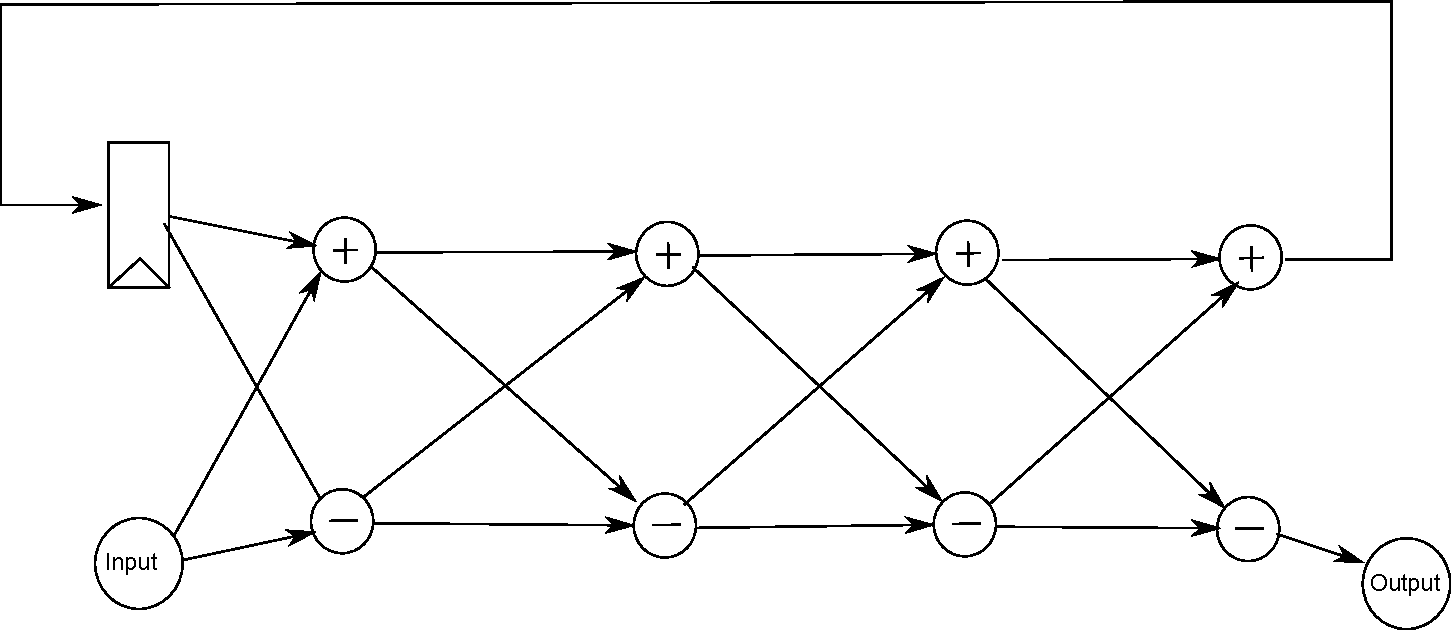
\includegraphics{figures/simpleFSM.pdf}}
\caption{{\bf Simple Finite State Machine Used For Evaluation}}
\label{fig:simpleFSM}
\end{figure}

\begin{table}[htb]
	\centering
	\resizebox{\columnwidth}{!}{
	\begin{tabular} 
		{ | l | r | r | r | }
		\hline
		& \textbf{Simple FSM} & \textbf{Simple RISC} & \textbf{Sodor} \\
		\hline \hline
		Number of Stages & $4$ & $4$ & $4$ \\
		\hline
		Max Unpipelined Combinational Path Delay & $125$ & $285$ & $380$ \\
		\hline
		Best Possible Pipelined Combinational Path Delay & $31.25$ & $71.25$ & $95$ \\
		\hline
		Actual Pipelined Combinational Path Delay & $50$ & $135$ & $175$ \\
		\hline
		Actual Pipelined Delay / Best Possible Pipelined Delay & $1.6$ & $1.89$ & $1.84$ \\
		\hline
	\end{tabular}
	}
	\caption{{\bf Pipelined Design Delay Data} The delays are obtained from analyzing the Chisel node graph pre synthesis. The delays are unitless because they are obtained from arbitrary mock delays assigned for the sake of independently testing the automatic pipeline placement tool}
	\label{fig:mock_delays}
\end{table}

%\begin{figure}[htb]
%\centering
%\resizebox{\columnwidth}{!}{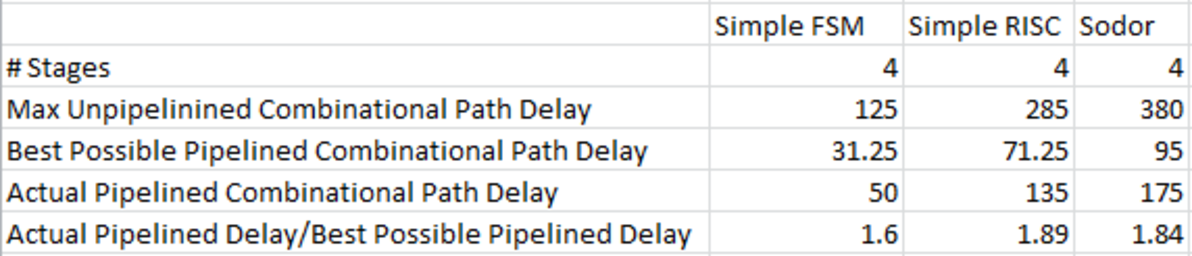
\includegraphics{figures/mock_delay_stats.pdf}}
%\caption{{\bf Pipelined Design Delay Data} The delays are unit less they are arbitrary units used for the sake of independently testing the automatic pipeline placement.}
%\label{fig:mock_delays}
%\end{figure}

We first want to evaluate the automatic pipeline placement independently from the Chisel Backannotation. Thus, we first run a very simple finite state machine (Figure \ref{fig:simpleFSM}.), a simple RISC processor(only implements control transfer and arithmetic operations and has no data memory access), and the Sodor processor through the automatic pipeline tools using mock delay numbers. Every Chisel Op node is give a mock delay of 5 and all other Chisel nodes are given mock delays of 0. Delay data is obtained by analysing the final Chisel graph after the automatic pipelining tool finishes placing the pipeline registers. For each example, we can obtain the best possible pipelined combinational path delay by dividing the maximum unpipelined combinational path delay by the number of pipeline stages. Then we can compare the actual pipelined combinational path delay against this best possible pipelined combinational path delay to get an idea of how well the automatic register placement is doing. We should not expect the tool to match the best possible pipelined combinational path delay because combinational logic nodes are not arbitrarily divisible and do not have uniform delays.

As seen in Table \ref{fig:mock_delays}, the automatic pipeline tool achieves relatively good  placement on a very simple finite state machine. At a glance, it seems that the tool should be able to achieve the best possible pipelined delay because there are 4 pipeline stages and there are 4 identical levels of logic. However, there are hidden muxes generated on the write port of the register in the Chisel node graph and the automatic pipelining tool cannot move pipeline registers across these hidden muxes. Thus, the achieved result matches our expectations.

The tool achieves slightly worse placement on the simple RISC processor ad the Sodor processor. This trend is explained by the fact that the automatic pipelining tool is more constrained on where it can place the pipeline registers on the more complex designs. Several things constrain the placement of the pipeline registers:

{\bf (1)} 
As discussed previously, the tool is not allowed to move IO nodes across pipeline stage boundaries. In more complex designs, there are more IO nodes and they prevent not only themselves, but also their inputs and consumers from being freely placed by the automatic pipelining tool. In the case of input nodes, its consumer nodes must be placed at a stage {\tt >=} the stage of the input node. In the case of output nodes, its input nodes must be placed at a stage {\tt <=} the stage of the output node.

{\bf (2)}  
The automatic pipelining tool cannot put pipeline registers in the middle of large black box modules such as caches. Thus, if the delay across the black box module is the critical path delay, the tool cannot reduce the critical path delay any further. The simple finite state machine does not use any black box modules while the more complex designs do.

{\bf (3)} 
The automatic pipelining tool cannot put pipeline registers between the input and output muxes of the read and write ports of array memories. In some designs, these read and write ports of array memories is a significant portion of the unpipelined critical path delay and thus the tool is unable to reduce the critical path delay below the propagation delay through the read and write ports of the array memories. The simple finite state machine does not use any array memories while the more complex designs each have an array memory for the register file.

Given these constraints, the automatic pipeline placement does a reasonable job placing the pipeline registers.
\subsection{Combined Tool Results}
\begin{table}[htb]
	\centering
	\resizebox{\columnwidth}{!}{
	\begin{tabular} 
		{ | l | r | r | r | }
		\hline
		& \textbf{Simple FSM} & \textbf{Simple RISC} \\
		\hline \hline
		Number of Stages & $2$ & $2$ \\
		\hline
		Max Unpipelined Combinational Path Delay & $0.9943$ & $0.5215$ \\
		\hline
		Best Possible Pipelined Combinational Path Delay & $0.49715$ & $0.26075$ \\
		\hline
		Actual Pipelined Combinational Path Delay & $0.5703$ & $0.5215$ \\
		\hline
		Actual Pipelined Delay / Best Possible Pipelined Delay & $1.15$ & $2$ \\
		\hline
	\end{tabular} }
	\caption{{\bf 2 Stage Pipelined Design Delay Data} The delays are in units of ns and are obtained from post-synthesis data.}
	\label{fig:comb_delays2}
\end{table}

\begin{table}[htb]	
	\resizebox{\columnwidth}{!}{
	\begin{tabular} 
		{ | l | r | r | r | }
		\hline
		& \textbf{Simple FSM} & \textbf{Simple RISC} \\
		\hline \hline
		Number of Stages & $3$ & $3$ \\
		\hline
		Max Unpipelined Combinational Path Delay & $0.9943$ & $0.5215$ \\
		\hline
		Best Possible Pipelined Combinational Path Delay & $0.3314$ & $0.1738$ \\
		\hline
		Actual Pipelined Combinational Path Delay & $0.418$ & $0.5215$ \\
		\hline
		Actual Pipelined Delay / Best Possible Pipelined Delay & $1.26$ & $3$ \\
		\hline
	\end{tabular} }
	\caption{{\bf 3 Stage Pipelined Design Delay Data} The delays are in units of ns and are obtained from post-synthesis data.}
	\label{fig:comb_delays3}	
\end{table}

\begin{table}[htb]	
	\resizebox{\columnwidth}{!}{
	\begin{tabular} 
		{ | l | r | r | r | }
		\hline
		& \textbf{Simple FSM} & \textbf{Simple RISC} \\
		\hline \hline
		Number of Stages & $4$ & $4$ \\
		\hline
		Max Unpipelined Combinational Path Delay & $0.9943$ & $0.5215$ \\
		\hline
		Best Possible Pipelined Combinational Path Delay & $0.248575$ & $0.130375$ \\
		\hline
		Actual Pipelined Combinational Path Delay & $0.418$ & $0.5215$ \\
		\hline
		Actual Pipelined Delay / Best Possible Pipelined Delay & $1.68$ & $4$ \\
		\hline
	\end{tabular} }
	\caption{{\bf 4 Stage Pipelined Design Delay Data} The delays are in units of ns and are obtained from post-synthesis data.}
	\label{fig:comb_delays4}	
\end{table}

%\begin{figure}[htb]
%\centering
%\resizebox{\columnwidth}{!}{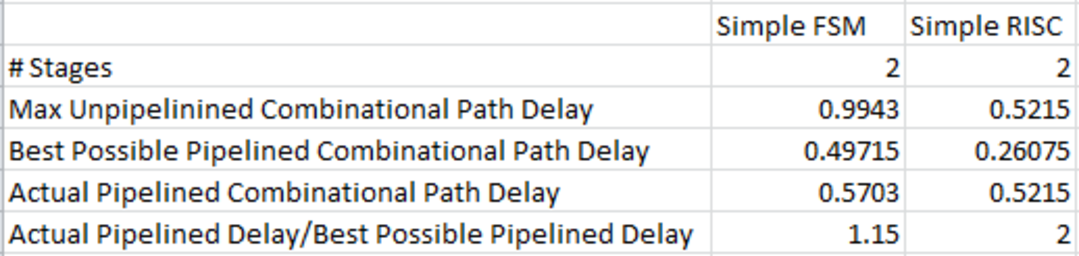
\includegraphics{figures/combined_delay_stats2.pdf}}
%\caption{{\bf 2 Stage Pipelined Design Delay Data} The delays are in units of ns.}
%\label{fig:comb_delays2}
%\end{figure}
%\begin{figure}[htb]
%\centering
%\resizebox{\columnwidth}{!}{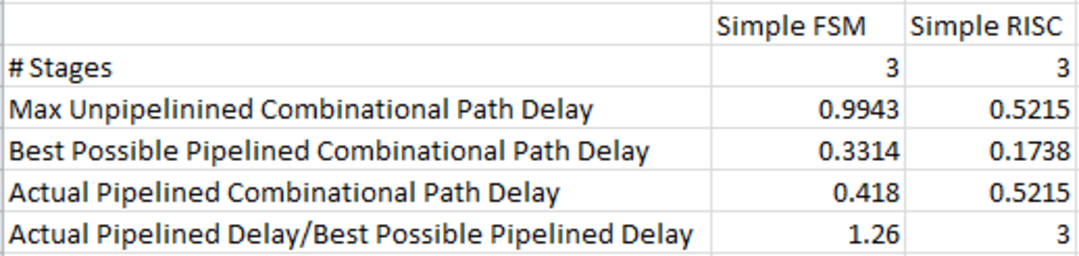
\includegraphics{figures/combined_delay_stats3.pdf}}
%\caption{{\bf 3 Stage Pipelined Design Delay Data} The delays are in units of ns.}
%\label{fig:comb_delays3}
%\end{figure}
%\begin{figure}[htb]
%\centering
%\resizebox{\columnwidth}{!}{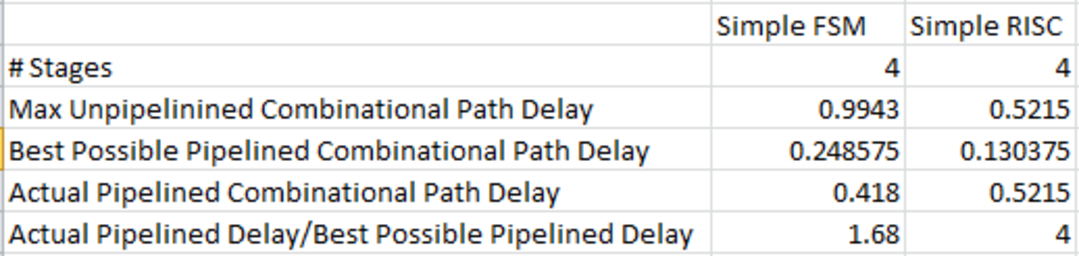
\includegraphics{figures/combined_delay_stats4.pdf}}
%\caption{{\bf 4 Stage Pipelined Design Delay Data} The delays are in units of ns.}
%\label{fig:comb_delays4}
%\end{figure}

We now evaluate the performance of the automatic pipeline placement function when using real delay data obtained from Chisel backannotation with the same metrics as the above section. The delay data is obtained by running the simple finite state machine and the simple RISC processor through the full combined tool flow involving the backannotation, the automatic pipelining tool, and finally synthesis. Synthesis is run with gate level optimizations turned off because we want to try to preserve a one to one mapping between the gate netlist and the Chisel node graph. We do not use the Sodor processors in the evaluation because we are unable to obtain delay data from them as they contain very large unsynthesizable scratchpad memories. We do not use post-place and route data because they introduce extra noise into the delay data due to how non-predictable layout patterns affect wire delays.

Table \ref{fig:comb_delays2}, Table \ref{fig:comb_delays3}, and Table \ref{fig:comb_delays4} show that the automatic pipelining tool performs very well on 2 and 3 stage versions of the simple finite state machine, with actual pipelined combinational path delays being very close to best possible pipelined combinational delays. This shows that given a sufficiently unconstrained design, automatic pipeline placement is able to do a good job when integrated with the real delay data provided by Chisel backannotation. Once again, intuition from looking at the simple finite state machine tells us that the tool should be able to perfectly balance the pipeline in the 4 stage implementation. However this is not true in reality because the output nodes have different input capacitances than the adders and subtractors in the design. In this case, the tool placed pipeline registers between each adder subtractor pair like we expect, but the delay from the final subtractor to the output node is the critical path due to the high input capacitance of the output node. Thus, the performance of the automatic pipeline placement tool on the 4 stage design is still a reasonable result.

Table \ref{fig:comb_delays2}, Table \ref{fig:comb_delays3}, and Table \ref{fig:comb_delays4} show that the automatic pipelining tool performs very poorly for the simple RISC processor. In fact, the critical path delay is the same for the 2,3, and 4 stage versions of the design. This is caused by constraint (3) described in \ref{auto_result}. In this case the critical path of the simple RISC processor is dominated by the muxes in the read port of its register file. The automatic pipelining tool has no way to place pipeline registers between these muxes, so the critical path delay is identical for the 2,3, and 4 stage designs.


\section{Conclusion and Future Work}
In this paper, we have improved the existing automatic pipelining tool in Chisel by adding functionality that allows the tool to automatically find a close-to-optimal placement of the pipeline registers with minimal manual specification. The improved Chisel automatic pipelining tool allows the designer to have to only label a small subset of the Chisel graph nodes in his design and automatically obtain a pipelined design that has close-to-optimal pipeline register placement based on real delay data gathered from Chisel backannotation. This presents a step towards further decreasing design effort for pipelining designs over the exisiting automatic pipelining tool.

The results of the Chisel backannotator show that it can calculate accurate critical path delays of most of designs in the Chisel tutorial except some designs such as Adder, BasicALU, and Risc. However, it does not mean each Chisel graph node has the exact delay numbers due to the arrival time estimation for missing signals, which may make the automatic pipelining tool yield non-optimal results. In addition, the delay numbers obtained from the backannotator are not realistic because the design is synthesized with simple design environment and constraints.  

To obtain realistic delay numbers, we will backannotate Chisel graphs with the delay information after placement and routing, which affects circuit timing significantly. To improve the Chisel backannotator's accuracy, we will develop more elaborated delay estimation for missing signals by mapping them to appropriate nets in the gate netlists. The observation is there are more nets than missing signals between two non-missing signals. We will use statical methods to map missing signals into their substitution nets. Also, the Chisel backannotator will have a mapping from logic cells to Chisel nodes, which is used to calculate not only delays, but area and power numbers.

Independent evaluation of the automatic pipeline register placement tool shows that the tool is capable of achieving reasonably optimal pipeline register placement for both simple finite state machines and more complex processor designs, when constraints on the tool are taken into consideration. When the tool is used with real delay data obtained with Chisel back annotation, the tool still achieves close-to-optimal pipeline register placement on designs that do not have their critical path dominated by paths that the tool cannot reach.

In future work, we plan to improve the automatic pipeline register placement by removing the restrictions on the tool preventing it from moving I/O nodes and architectural register read and write points. This will decrease the constraints on where the tool can place the pipeline registers and allow the tool to achieve more optimal pipeline register placements on complex designs. We also want to do a study of how the tool performs when it is combined with VLSI retiming tools.

\section*{Course Feedback}
\textbf{Donggyu:} This course was very helpful to understand the flow of VLSI designs. I had no background knowledge on VSLI CAD tools, but now, I'm familiar with Sysnopsys tools through labs and the project. It's also good opportunity to learn basic circuit backgrounds and VLSI design patterns which I'm weak at. I'm generally satisfied with this course. One thing I was not satisfied with is it takes extremely long time due to CAD tool running times. I'm not sure we have to execute DC in a topographical mode for the labs because we will run ICC later. I think we can reduce running times by excluding unnecessary design environment and constraints.
\bibliographystyle{abbrvnat}
\setlength{\bibsep}{0.0pt}
\renewcommand*{\bibfont}{\footnotesize}
\bibliography{references}

\end{document}
